%%%%%%%%%%%%%%%%%%%%%%%%%%%%%%%%%%%%%%%%%
% University Assignment Title Page
% LaTeX Template
% Version 1.0 (27/12/12)
%
% This template has been downloaded from:
% http://www.LaTeXTemplates.com
%
% Original author:
% WikiBooks (http://en.wikibooks.org/wiki/LaTeX/Title_Creation)
%
% License:
% CC BY-NC-SA 3.0 (http://creativecommons.org/licenses/by-nc-sa/3.0/)
%
% Instructions for using this template:
% This title page is capable of being compiled as is. This is not useful for
% including it in another document. To do this, you have two options:
%
% 1) Copy/paste everything between \begin{document} and \end{document}
% starting at \begin{titlepage} and paste this into another LaTeX file where you
% want your title page.
% OR
% 2) Remove everything outside the \begin{titlepage} and \end{titlepage} and
% move this file to the same directory as the LaTeX file you wish to add it to.
% Then add \input{./title_page_1.tex} to your LaTeX file where you want your
% title page.
%
%%%%%%%%%%%%%%%%%%%%%%%%%%%%%%%%%%%%%%%%%
%\title{Title page with logo}
%----------------------------------------------------------------------------------------
% PACKAGES AND OTHER DOCUMENT CONFIGURATIONS
%----------------------------------------------------------------------------------------

\documentclass[12pt]{article}
\usepackage[english]{babel}
\usepackage[utf8x]{inputenc}
\usepackage{amsmath}
\usepackage{graphicx}
\usepackage[colorinlistoftodos]{todonotes}
\usepackage[none]{hyphenat}
\usepackage{hyperref}
\setlength{\parindent}{0pt}
\usepackage{caption}
\frenchspacing

\begin{document}

\begin{titlepage}

\newcommand{\HRule}{\rule{\linewidth}{0.5mm}} % Defines a new command for the horizontal lines, change thickness here

\center % Center everything on the page

%----------------------------------------------------------------------------------------
% HEADING SECTIONS
%----------------------------------------------------------------------------------------

\textsc{\LARGE University Of Windsor}\\[1.5cm] % Name of your university/college
\textsc{\Large 60-367}\\[0.5cm] % Major heading such as course name
\textsc{\large Computer Networks}\\[0.5cm] % Minor heading such as course title

%----------------------------------------------------------------------------------------
% TITLE SECTION
%----------------------------------------------------------------------------------------

\HRule \\[0.4cm]
{ \huge \bfseries Botnet Research Paper}\\[0.4cm] % Title of your document
\HRule \\[1.5cm]

%----------------------------------------------------------------------------------------
% AUTHOR SECTION
%----------------------------------------------------------------------------------------

% If you don't want a supervisor, uncomment the two lines below and remove the section above
\Large \emph{Author:}\\
Quinn Perfetto - 104026025\\[3cm] % Your name

%----------------------------------------------------------------------------------------
% DATE SECTION
%----------------------------------------------------------------------------------------

{\large \today}\\[2cm] % Date, change the \today to a set date if you want to be precise

\vfill % Fill the rest of the page with whitespace

\end{titlepage}


\tableofcontents

\pagebreak

\section{Introduction}

A botnet is a private network of computers infected with malicious software which allows them to be controlled by an entity known as the \textbf{Command and Control (C\&C)}.
The infected computers, referred to as \textbf{zombies}, are generally unaware that they are members of the botnet. 
Botnets are most often used to send large quantities of spam emails and distribute denial of service attacks \cite{kapersky}.
Botnets provide the C\&C with the computing power of all zombies in the network while masking the identity of the true attacker.
\\ \\
As an analogy, imagine that you send an email to your 10 closest friends falsely claiming that a local ice cream store
is giving out free ice cream on a certain date.  Naturally these friends are excited and each of them forward this email
to their 10 closest friends.  This process continues, and soon enough thousands of people are under the impression
that they will be receiving free ice cream.
Your network of friends don't realize it, but they have just been turned into a botnet with the express purpose of shutting down the ice cream shop.
When the much anticipated date arrives, the store is flooded with customers demanding free sweets (it was advertised, after all).
Unable to handle the hoard of customers (zombies) the store is forced to shutdown for the day and focus their efforts in remedying the misunderstanding.
\\ \\
Who is to blame for the shop's loss in profits for the day?  The intent of the crowd was genuine,
and the continual forwarding of the email has made it virtually impossible to trace
it back to its source.  You were successfully able to harness the power of thousands
of people all while remaining anonymous.

\begin{center}
  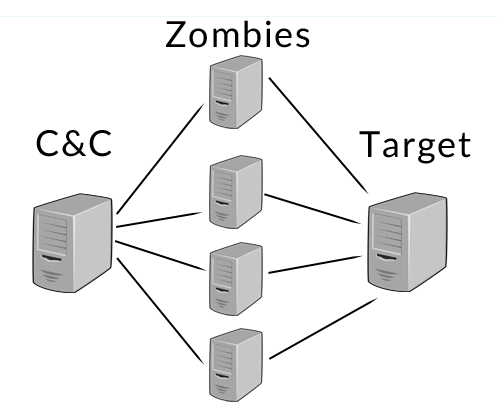
\includegraphics[width=0.5\textwidth]{assets/botnet_example.png}
  \captionof{figure}{An example of the C\&C commanding the zombies to attack \textit{Target.}}
  \label{fig:botnet_example}
\end{center}

\section{Motivation}
\subsection{Political}
\subsection{Economic}
\subsection{Curiosity}

\section{Mechanics}

\subsection{The Life Cycle of a Botnet}
\subsubsection{Recruitment}
In order to be effective, a botnet must have a large collection of zombies within its network of control.
Botnet creators commonly use a type of malware called a \textbf{worm} to recruit new members
\cite{lifecycle}.
Worms can be distinguished from other forms of malware by their ability to self replicate
in order to spread to other computers on the same network \cite{virustypes}.
This property is attractive to botnet creators as it promotes rapid spreading of the virus across
multiple hosts, and each new zombie adds an additional degree of separation from the source.
The techniques used to infect the initial set of zombies are consistent with
those used in general virus spreading.  These techniques may include social engineering,
embedding the virus in email attachments, and \textit{something else}.
Once a new zombie is infected it "phones home" to the C\&C to register
itself as a member of the botnet, and then lays dormant awaiting a command
\cite{topology}.

\subsubsection{Command Propagation}
Once a sizeable network of zombies is formed the C\&C needs a mechanism for
relaying commands and updates. Interestingly, many of the different network topolgies
used to accomplish this bear similarities to those used in non-malicious settings.

\paragraph{Star \cite{topology}}
A single C\&C point of contact performs all communication with the members
of the botnet. This type of topology can be observed in Local Area Networks
where all computers are connected to the internet through a single router. As a
result it typically does not scale well with an increased number of zombies.

\begin{center}
  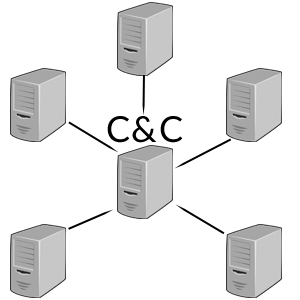
\includegraphics[width=0.5\textwidth]{assets/startopo.png}
  \captionof{figure}{A botnet with a star communication topology.}
  \label{fig:star_topo_fig}
\end{center}

\begin{tabular}{p{8cm} | p{8cm}}
  \textbf{Pros} & \textbf{Cons} \\ \hline
  \textbullet{}Simple to implement                                    & \textbullet{}Single point of failure \\
  \textbullet{}Allows for rapid communication of commands and updates & \textbullet{}Large amount of network traffic traveling to and from single location\\
                                                                      & \textbullet{}Easier to locate C\&C
\end{tabular}

\paragraph{Multiserver \cite{topology}}
Multiple interconnected C\&C servers coordinate to distribute messages to the zombies.
Thoughtful geographical placement of these C\&C servers can reduce latency across
large distances.  This technique can be seen at the network core where each
ISP provides internet connection to a small subset of the population, with support for
inter-ISP communication accross long distances.

\begin{center}
  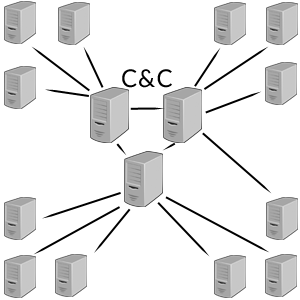
\includegraphics[width=0.5\textwidth]{assets/multiservertopo.png}
  \captionof{figure}{A botnet with a multiserver communication topology.}
  \label{fig:mulitserver_topo_fig}
\end{center}

\begin{tabular}{p{8cm} | p{8cm}}
  \textbf{Pros} & \textbf{Cons} \\ \hline
  \textbullet{}Reduced load on each C\&C                    & \textbullet{}Difficult Initial Setup \\
  \textbullet{}Zombies can fail over incase of a C\&C crash & \textbullet{}Complicated Coordination\\
  \textbullet{}Optimized for long distance communication    & \\
\end{tabular}

\paragraph{Peer to Peer (P2P) \cite{topology}}
No centralized C\&C, commands can be injected into the botnet at any zombie.
Each zombie that recieves a command will then fan it out to all known peers.
Generally these commands are signed with some sort of secret key to verify they
are coming from an authoritative source \cite{topology}. Botnets orgainized
this way are extremely difficult to shutdown as they generally implement redundant
connections \cite{topology}.  This type of topology is most famously used in BitTorrent,
a service where peers can directly share files with one another without the need for a central
repository.

\begin{center}
  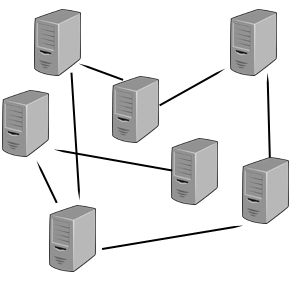
\includegraphics[width=0.5\textwidth]{assets/p2ptopo.png}
  \captionof{figure}{A botnet with a P2P communication topology.  Note the lack of explicit C\&C.}
  \label{fig:p2p_topo_fig}
\end{center}

\begin{tabular}{p{8cm} | p{8cm}}
  \textbf{Pros} & \textbf{Cons} \\ \hline
  \textbullet{}No central point of contact & \textbullet{}Command propagation could be slow \\
  \textbullet{}Difficult to shutdown       & \textbullet{}Members can be discovered by observing fanout messages\\
                                           & \textbullet{}Infected users may notice spikes in bandwidth usage\\
\end{tabular}

\subsubsection{Attack}

\subsection{Techniques For Remaining Undetected}
\subsubsection{P2P Command Propagation}
\subsubsection{Encrypted Protocols}

\section{Botnet Detection/Mitigation}

\section{Analysis of Historial Botnets}

\subsection{The Morris Worm}
First semblance of a botnet.  Changed the internet's outlook on security.

\subsection{Conficker}

\subsection{Stuxnet}

\subsection{Dyn DNS}
Discuss problems with IoT.

\section{Legal/Consenual Botnets}
Research, lulz lazor, etc.

\pagebreak
\begin{thebibliography}{1}

  \bibitem{kapersky} Kapersky Lab {\em What is a Botnet Attack?}  https://usa.kaspersky.com/internet-security-center/threats/botnet-attacks.

  \bibitem{lifecycle} R. A. Rodriguez-Gomez {\em Analysis of botnets through life-cycle} 2011:
  Proceedings of the International Conference on Security and Cryptography.

  \bibitem{virustypes} Cisco {\em What Is the Difference: Viruses, Worms, Trojans, and Bots?}  http://www.cisco.com/c/en/us/about/security-center/virus-differences.html.

  \bibitem{malwareprop} MR Faghani {\em Malware Propagation in Online Social Networks} 2009:
  Proceedings of the 4th IEEE International Conference on Malicious and Unwanted Software.
  
  \bibitem{topology} G Ollmann {\em Botnet Communication Topologies} 2009:
    \url{https://www.damballa.com/downloads/r_pubs/WP_Botnet_Communications_Primer.pdf}.

\end{thebibliography}

\end{document}
